\documentclass[]{article}

%opening
\title{MLP Coursework 4}
\author{Eskil Joergensen}
\date{\today}

\usepackage[parfill]{parskip}
\usepackage{pgfgantt}
\usepackage{multicol}
\usepackage{multirow}
\usepackage{tikz}
\usepackage{pgfplots}
\newcommand*\rot{\rotatebox{90}}
\usepackage{graphicx}
\graphicspath{ {images/} }

\usepackage{amsmath}

\usepackage{booktabs}
\usepackage[font={small,it}]{caption}

\begin{document}

\maketitle

\section{Introduction}

Fully connected neural networks are trained at a relatively low computational cost, and they have been used in machine learning for quite some time. However, current state-of-the-art networks are all convolutional neural networks (CNNs) \cite{long2015fully}. The high performance is (typically) achieved as the kernels in the convolutional layers extract features from the input data via their spacial locality. A common use case is object recognition in images, but can also be used in other tasks such as natural language processing \cite{Collobert}. 

Preliminary work has been done on the same data set using a fully connected neural network. More details are presented in the Background section (\ref{background}) below. 

CNNs introduce a significantly larger number of weights and connections, compared to a fully connected network, which means the parameters of the network must be carefully tuned to ensure adequately successful training. 

This report presents a series of experiments set to investigate how some key components of a CNN affect it's overall performance during training. Furthermore, the (optimal) findings from each experiment are integrated into the network for the subsequent experiments, trying to improve the performance of the network as much as possible. The following aspects of the CNN are investigated:

\begin{itemize}
	
	\item How does the size of kernels and number of feature maps in the convolutional layers affect the training? Time, performance, computational resources
	
	\item How does the choice of activation function impact the performance of the network?
	
	\item What type, and magnitude, of regularization is needed to overcome potential over-fitting of the CNN?
	
\end{itemize}

optimize the training performance of a CNN on a image classification task, using the CIFAR 10 dataset \cite{cifar10}. In addition to improving the overall performance of the training of the network, the experiments were guided by a goal of 70\% accuracy on the test data set. As a result, the methodology and incremental improvements to the model were made on these grounds. 

\subsection{Background} \label{background}

Preliminary experiments have been conducted on the same data, using a fully connected neural network. The network was trained using a variety of activation functions, hidden layer depths and widths as well as learning rate scheduler. 

\subsubsection{Activation Functions}

Four activation functions were compared. The logistic sigmoid $f(x)=\frac{1}{1+e^{-x}}$, the hyperbolic tangent $f(x)=tanh(x)$ the rectified linear (ReLu) $f(x)=max(0,x)$ and the exponential linear unit (ELU):

\begin{equation} \label{eq:elu}
f(x) = \begin{cases}
x &\text{if $x >$ 0}\\ \alpha (\text{exp}(x) - 1) &\text{if  $x \leq$ 0}
\end{cases}
\end{equation}

where \(\alpha\) is a hyperparameter that decides the range of negative values for which the activation function saturates.

The results showed that the ELU activation function outperformed the other three, with a final training and validation set accuracy of 66.9 \% and 50.5\% respectively. 

\subsubsection{Hidden layers}

\subsubsection{Learning Rate Schedule}

\section{Network Architecture}



\section{Methodology}

2. Treatment for the object (what do to object)
3. Procedure to collect data
4. Procedure to analyze data


\subsection{The Network Architecture}

A neural network with two convolutional and two fully connected hidden layers was chosen for this study. The network also had two max pooling layers, one after each convolutional layer, as well as a 10-way softmax output classification. 

Why this model?

\begin{figure}[h]
	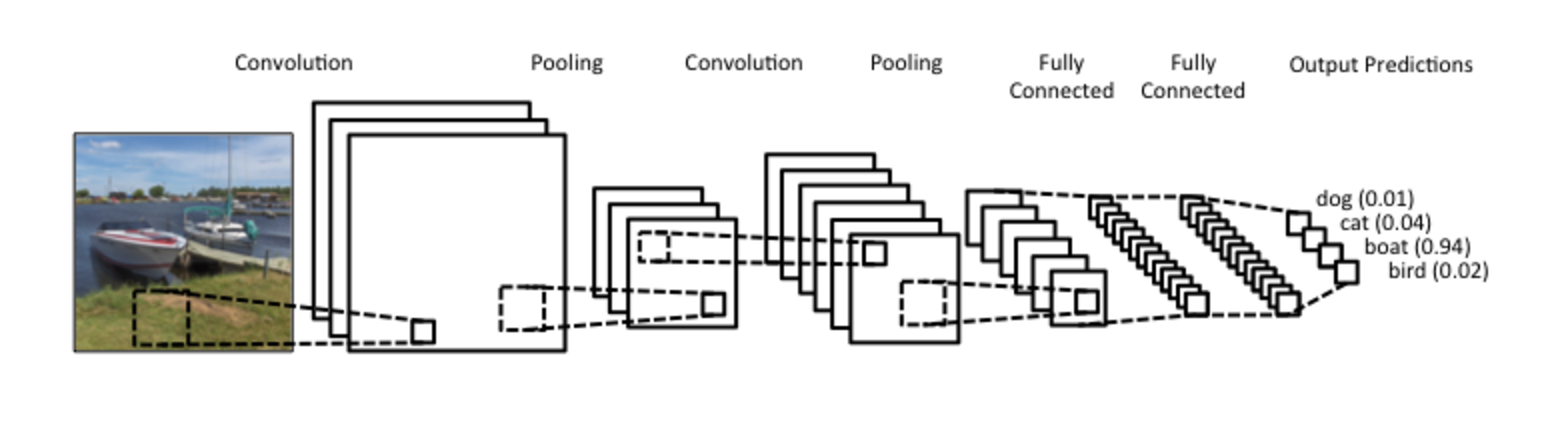
\includegraphics[width=\textwidth]{conv}
	\caption{Showing a visual representation of the model used, from TensorBoard.}
	\label{conv}
	\centering
\end{figure}

\subsubsection{Convolutional Layer}

The convolution was implemented using the \texttt{tf.nn.conv2d} method from TensorFlow (tf) with stride of 1 and no padding (\texttt{padding='SAME'}). The convolution operation was executed on the layer inputs together with the kernels (using the specified stride and padding). Both the layer inputs and the kernels were TensorFlow tensors, and the result of the convolutional operation was also a TensorFlow tensor. 

The biases were added to the tensor after the convolution. In the convolutional layers where batch normalization was specified, ... . Finally, an activation function was applied to the tensor, before passing the output on to the next layer. 

A truncated normal distribution was use to initialize the kernels, and the biases were initialized to zero. See Section \ref{weights}, Weight and Biases, for the specific implementation in TensorFlow. 

\subsubsection{Fully Connected and Output prediction Layer}

The fully connected and the classification output layers were implemented using the same class, as only a few factors separate the behavior of the two. A constant halving of the number of hidden units were integrated into all the fully connected layers, except the output prediction layer which had a 10-was output.

The weights and biases were initialized in the same as mentioned for the convolutional layers, only the weights for the affine layers were two dimensional. 

Finally, the inputs were multiplied with the weights using \texttt{tf.matmul} ,before the biases were added to the tensor. For the final classification layer this tensor would be returned, otherwise an activation function would be applied before returning the tensor.

\subsubsection{Pooling Layer}

The max pooling layer was implemented using the \texttt{tf.nn.max\_pool} method from TensorFlow. Each pooling layer used a 3 by 3 window for the sampling, and a stride of 2. Similarly to the convolutional layer the pooling layer used no padding, \texttt{padding='SAME'} in TensorFlow. 

\begin{figure}[h]
	\centering
	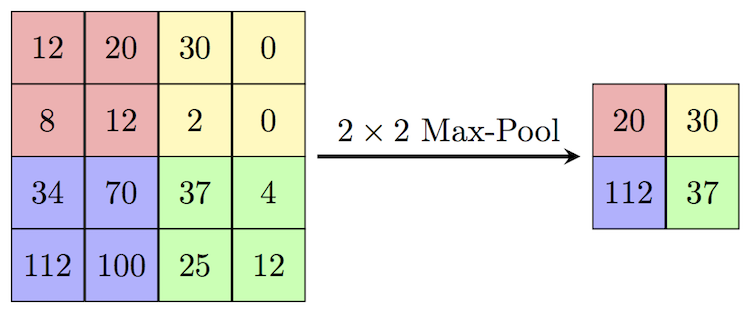
\includegraphics[width=0.6\textwidth]{pool}
	\caption{Showing an example of a 2x2 max pool operation.}
	\label{pool}
	\centering
\end{figure}

\subsubsection{Dropout Layer}

The dropout layer was implemented using \texttt{tf.nn.dropout(inputs, keep\_prop)}, and will keep each element in the input tensor with a probability of \texttt{keep\_prob}. 

\subsubsection{Batch Normalization}

The batch normalization of the convolutional layer was achieved with the \texttt{tf.nn.max\_pool} method from TensorFlow. Batch normalization transforms its input to zero mean and unit variance. By statistical analysis the batch normalization normalizes the inputs of a transformation layer. Equation \ref{batch_eq} shows how the inputs \(x_i\) are normalized

\begin{equation} \label{batch_eq}
BN(x_i) = \gamma_i \Big( \frac{x_i - \mu_i}{\sqrt{\sigma_i^2 + \epsilon}} \Big) + \beta_i
\end{equation}

where \(\mu_i\) is the batch mean, \(\sigma_i^2\) is the batch variance, \(\gamma_i\) is a scale factor and \(\beta_i\) is a shift factor. \(\gamma_i\) was set to 1.0, \(\beta_i\) to zero and \(\epsilon\) to 1e-3. The batch mean and variance was obtained from the inputs using \texttt{tf.nn.moments}. 


\subsubsection{Weights and Biases} \label{weights}

The weights used in both the convolutional and fully connected layers were initialized using a truncated normal distribution. The values were distributed with zero mean and a standard deviation of 0.1. Values more than two standard deviations away from the mean were dropped. The distributions were initialized with the \texttt{tf.truncated\_normal} method. 

The biases used were all initialized to zero using the tf.zeros method. Additionally, the weights and biases were added to the TensorFlow. graph using  tf.Variable().

\subsection{Experimental Procedure}

The procedure used to tune the performance of the network involved three stages. During the initial stage the network was trained for few epochs, with a coarse spread of hyper parameter and multiple algorithms were tested during this phase. The overall results from the initial trials informed the finer range of parameters used for additional training and further tuning of hyper parameters. The second stage involved longer training. The third stage, before the final testing, the model was trained for significantly longer, and only three varieties of the model were used. 


The default baseline model used has two convolutional layers, two fully-connected layers and finally a softmax classification layer. The network also had two 2x2 pooling layers after each convolutional layer. 

Instead of a learning rate scheduler, the Adam adaptive learning rate optimizer was used throughout the investigation. The optimizer was used with varying learning rates, but with beta1=0.9, beta2=0.999 and epsilon = 1e-8. (default parameters) 


\subsubsection{Activation Functions}

Initially the model was trained using three learning rates, with the four activation functions used in the preliminary experiments: ReLu, Elu, Tahn and Sigmoid. These were tested with a learning rate of 0.0005, 0.003 and 0.01, and the network was trained for 5 epochs. The relatively large, non-uniform spread of the learning rate was chosen intentionally to observe how the activation functions would react to the rates.

After the initial trials, the best two activation functions were kept for further experimentation, and the other two were discarded. The worst learning rate for each of the remaining activation functions was also replaced with another learning rate, trying to narrow down the region of learning rates for which the training of the network performs better. For the second round of trials, the network was trained for 10 epochs. 

The second round informed the activation function to be used for the last round, and again the learning rates were narrowed down further. The last set of trials, for the activation functions, the network was trained for 20 epochs. The learning rate that resulted in best performance was then used for the during the later experiments. 

The activation functions and learning rates were tested using two convolutional layers with 3x3 kernels and 24 feature maps. The model also had a 3x3 pooling layer with stride of two after each convolutional layer. After the tensors were flattened, the network had two fully connected layers before a final softmax classification layer. The network used the Adam optimizer. 

\subsubsection{Filter Sizes and Feature Maps}

The kernels are responsible for extracting features from the input data, and their sizes as well the the number of feature maps output will affect the performance of a network. 

The network was trained using a number of combinations of kernel sizes and feature maps in each of the convolutional layers. The size of kernels were 3, 5 and 7, whereas the number of feature maps were 16, 24 and 32. Here as well, the best combination was chosen for the following trials.

The architecture and training parameters remained the same as for the experiments on the activation functions, except the ELU activation function was used with a learning rate of 0.0004. 

\subsubsection{Regularization and Normalization}

Without any normalization or regularization significant over-fitting can occur during training of the network. 

As with the previous experiments, short trials were run using coarse set of parameters. Using three nested loops, the network was trained using eight different combinations of batch normalization, drop out and L2 weight decay. The batch normalization added to the convolutional layers were either true or false, the L2 decay was none or 0.0005 and the keep probability of the dropout layers were either 1.0 (keep all) or 0.5. The network was trained for 5 epochs during the first set of trials. 



introduced dropout and data augmentation

trained for 40 epochs
 
 
\section{Results and Discussion}

\subsection{Activation Functions}

After the model was trained with all four transformation functions, the ReLu and ELU performed significantly better than the sigmoid and hyperbolic tangent. The first 5 epoch trial showed that a learning rate of 0.01 was too large, and resulted in high total error and low accuracies around 0.1, which meant the final classifications were merely guesses. The lowest learning rate, 0.0005, resulted in the highest accuracies across all the activation functions, and the ReLu trial had a final validation accuracy of 70.3\%. 

During the second round of trials, the network was trained with the ReLu and ELU activation functions, with learning rates of 0.0009 and 0.0001. After training the network for 10 epochs, the performance decreased for both activation functions, suggesting the better learning rates were closer to 0.0005. The final trial was then run with learning rates of 0.0004 and 0.0007. 

The last set of trials gave very similar results, see Figure \ref{ac_res}. The highest validation accuracy was 71.6\%, by ELU with the learning rate of 0.0004, and the lowest was 69.7\% by ReLu with the learning rate of 0.0007. Although the validation accuracy was over 70\%, the training set accuracies were much higher, which indicates a high degree of over-fitting. The over-fitting was also reflected in the validation set errors, as can be seen in Figure. 

\begin{figure}[h]
	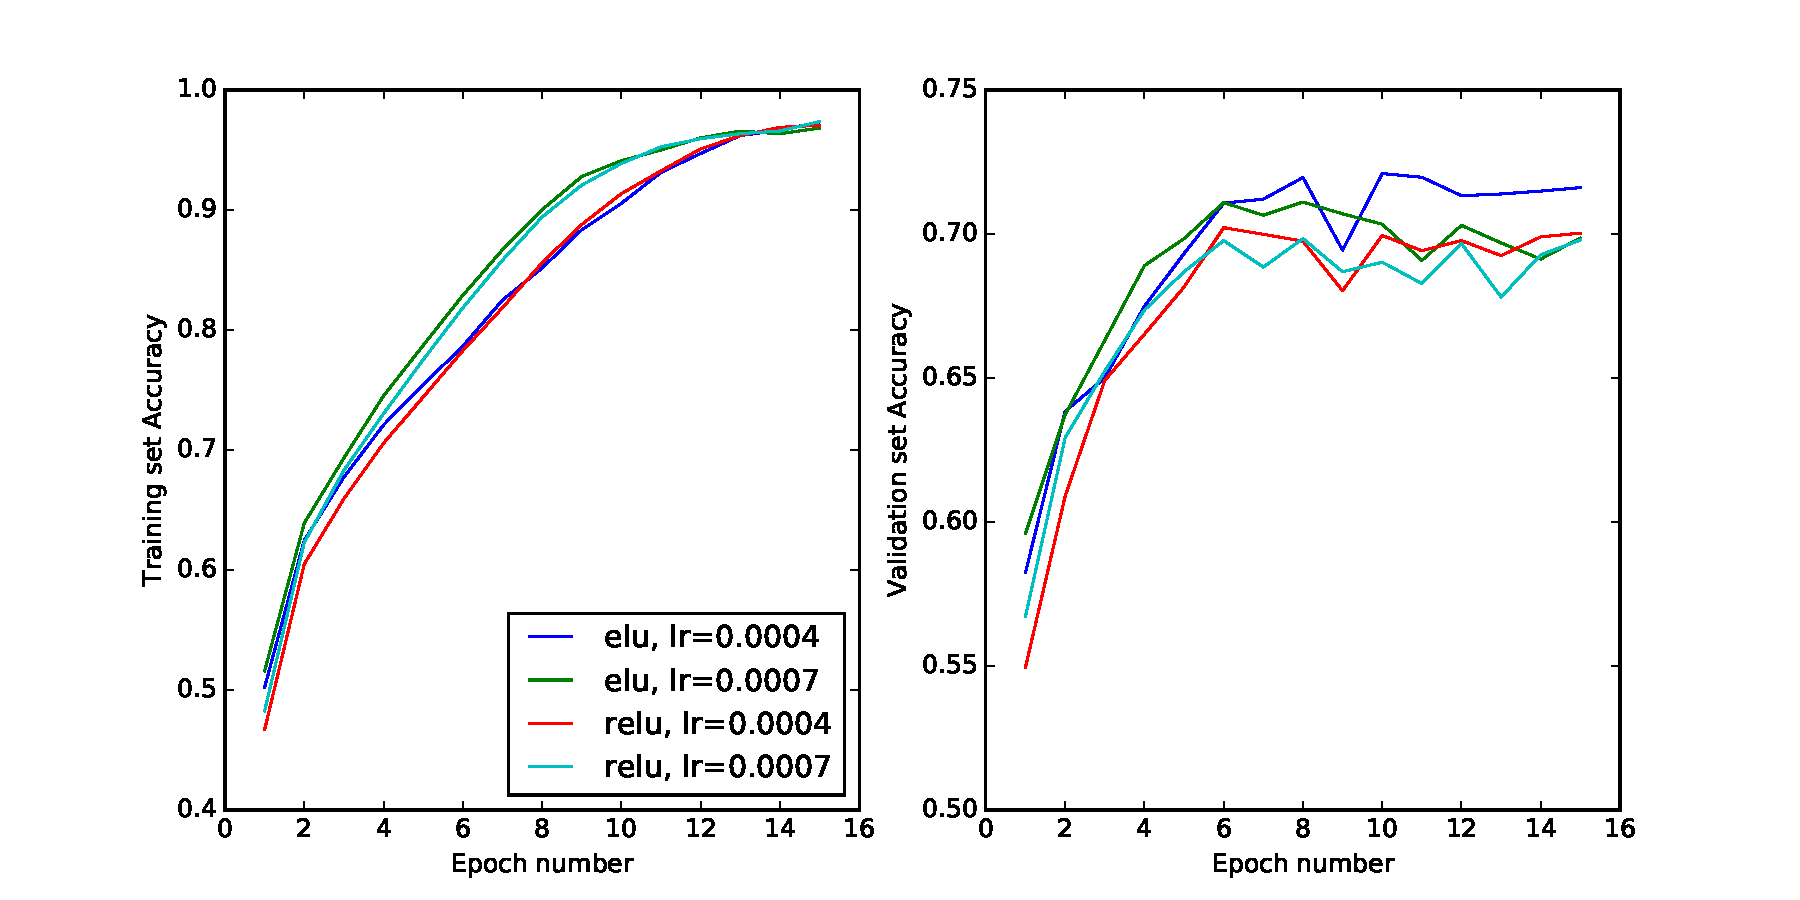
\includegraphics[width=\textwidth]{ac_res}
	\caption{Showing a visual representation of the model used, from TensorBoard.}
	\label{ac_res}
	\centering
\end{figure}

\subsection{Filter Sizes and Feature Maps}

The number of feature maps had a greater impact on the training performance, compared to the size of the kernels. As shown in Figure , the three best performing trials were all using convolutional layers with 32 feature maps. 

\begin{table}[h]
	\centering
	\caption{Showing the training execution time, in minutes, for 5 epochs for different kernel sizes and number of feature maps in the convolutional layers.}
	\label{my-label}
	\begin{tabular}{@{}ccccc@{}}
		\toprule
		\multicolumn{2}{c}{Feature Maps} & 16 & 24 & 32 \\ \midrule
		\multirow{3}{*}{\rot{Size}} & \multicolumn{1}{c|}{3x3} & 12.5 & 19.1 & 27.0 \\
		& \multicolumn{1}{c|}{5x5} & 22.5 & 34.6 & 49.1 \\
		& \multicolumn{1}{c|}{7x7} & 39.9 & 57.9 & 67.0 \\ \bottomrule
	\end{tabular}
\end{table}



\subsubsection{Regularization and Normalization}

\section{Conclusion}

\section{Future Work}


\clearpage
\medskip
\bibliographystyle{IEEEtran}
\bibliography{ref.bib}

\end{document}
